\documentclass{article}
\usepackage[portuguese]{babel}
\usepackage[a4paper, top=3cm, bottom=2cm, left=2.5cm, right=2.5cm]{geometry}
\usepackage{blindtext}
\usepackage{float}
\usepackage{datetime}
\usepackage{csvsimple}
\usepackage[T1]{fontenc}
\usepackage{graphicx} 
\usepackage{xcolor}
\usepackage{soul} 
\usepackage{tcolorbox}
\usepackage{indentfirst}
\usepackage{fancyhdr}  
\usepackage{caption}
\usepackage{enumitem}
\usepackage{titlesec}
\usepackage{titletoc}
\usepackage{hyperref}


\newcommand{\annotationbox}[3]{
    \definecolor{currentcol}{named}{#3} 
    \begin{tcolorbox}[colback=currentcol!5!white, colframe=currentcol!75!black, title={#1}]
        {#2}
    \end{tcolorbox}
}

\newcommand{\theauthor}{Grupo - Número}
\newcommand{\thetitle}{Tema do trabalho}


\newcommand{\highlight}[1]{{\sethlcolor{yellow}\hl{#1}}}   

\pagestyle{fancy}  
\fancyhf{}  
\rhead{\theauthor} 
\lhead{Tema do trabalho}  
\cfoot{\thepage} 


\begin{document}



\begin{titlepage}
    \begin{center}
        \begin{figure}[htb!]
            \centering
            
\includegraphics[width=150mm]{../images/ifsc_logo.jpg}
        \end{figure}
        \vspace{20pt}
        \LARGE{\textbf{Universidade de São Paulo}}\\
        \LARGE{Instituto de Física de São Carlos}\\

        \vspace{150pt}

        
        \LARGE{\textbf{{\thetitle}}} 
        \\ 
        \textsc{\LARGE Subtema}
        \\
        
        
        \vspace{125pt}
        \begin{minipage}{\textwidth}
            \begin{flushleft} \large
                \textbf{Professor:}\\
                Professor\\[0.8cm]
                \textbf{Grupo - Número:}\\
                Johnny - Num USP
                \\
                Marry - Num USP
                \\
                Paul - Num USP
                \\
                George - NumUSP
                
                \end{flushleft}
                \end{minipage}\\[1 cm]
        \vspace{30pt}
        \vspace{\fill}  
        \Large {\today}

    \end{center}
\end{titlepage}

\newpage
\tableofcontents
\listoffigures

\newpage

\section{Citação Direta}
Geralmente o bibtext das citações
podem ser tirados do \href{https://www.books.google.com.br}{Google Livros}, para
transformar um pdf sem busca para um pesquisável, basta usar o site
\hyperlink{tools.pdf24.org/pt/ocr-pdf}{ToolsPDF24}, para algumas
citações longas é importante que tenha um highlight nas partes mais importantes

\begin{quotation}
    \highlight{I shall now teach you how to multiply the unknown
    numbers}, that is to say, the roots, one by the other, if
    they stand alone, or if numbers are added to them, or if
    numbers are subtracted from them, or if they are subtracted 
    from numbers; also how to add them one
    \begin{flushright}
        The Algebra of Mohammed Ben Musa\cite[p. 30]{khuwarizmi2022algebra} 
      \end{flushright}
    \end{quotation}


\section{Citação de Imagens}
Imagens retiradas da Wikipedia possuem uma citação bem fácil, basta pesquisar a 
imagem no WikiMedia commons e extrair a citação 

\begin{figure}[H]
    \centering
    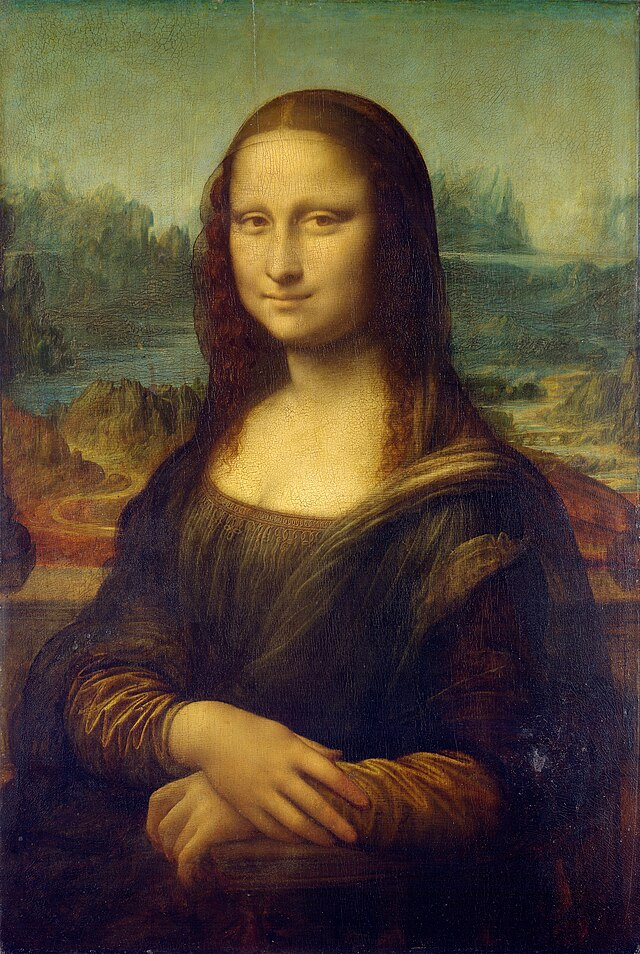
\includegraphics[width=50mm]{../images/monalisa.jpg}
    \caption{Leonardo da Vinci, Public domain, via Wikimedia Commons}
\end{figure}

Agora vamos citar uma imagem retirada de um Livro

\begin{figure}[H]
    \centering
    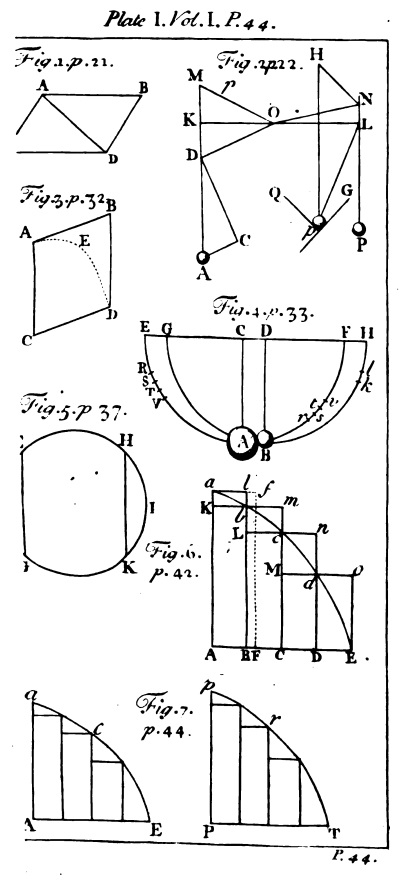
\includegraphics[width=50mm]{../images/newton_drawing.jpg}
    \caption{Esquemático feito por Newton \cite[Plate I.Vol.I.P.44.]{newton1729mathematical}}
\end{figure}


\bibliography{../bibliografia/referencias.bib}
\bibliographystyle{abbrv}


\end{document}
